\chapter{Diseño}

En este apartado se van a describir cada una de las herramientas, entornos y metodologías que se van a seguir a la hora de implementar el software del que se ha hecho el análisis y especificación en el capítulo anterior.
\bigskip

\section{Herramientas a utilizar}

Para el desarrollo se va a utilizar el lenguaje de programación M propio de MATLAB cuyo núcleo está desarrollado en C y Java. Es de propósito específico para la implementación de software matemático, que con el tiempo ha ido ampliando sus capacidades de desarrollo hasta convertirse en un lenguaje completo que puede crear interfaces gráficas mediante GUIDE, interconexión con dispositivos hardware, etc.
\bigskip

Cómo se ha comentado en capítulos anteriores se va a hacer uso de la toolbox MEDA que implementa una serie de herramientas estadísticas para el análisis exploratorio de datos y la visualización de los mismos en distintos tipos de gráficas. Dicha toolbox tiene la capacidad de análisis supervisados de datos con PLS, análisis no supervisados con PCA y las visualizaciones se hacen mediante Score plots, Loading Plots, gráficos Meda y oMEDA.
\bigskip

Dentro de MEDA-Toolbox para este proyecto se van a utilizar los módulos:
\bigskip

\begin{itemize}
	\item \textbf{Update\_iterative2.m:} Se encarga de generar la estructura Lmodel mediante análisis PCA o PLS según se le especifique, siguiendo el método "iterative" para BIG DATA. Es una modificación del módulo update\_iterative.m añadiendo una funcionalidad de salida de información mediante una consola o terminal propio de cada interfaz gráfica que se le pasa por argumento al módulo.
	\item \textbf{Update\_ewma2.m:} Hace lo mismo que el módulo anterior pero basándose
en el método EWMA, al igual que en el caso anterior es una modificación de update\_ewma.m para añadir la funcionalidad de la consola propia.
	\item \textbf{Score\_LPLS.m:} Generar un gráfico Score Plots con BIG DATA y siguiendo el modelo PLS.
	\item \textbf{Scores\_LPCA.m:} Generar un gráfico Score Plots con BIG DATA y siguiendo el modelo PCA.
	\item \textbf{Meda\_LPLS.m:} Genera una matriz MEDA y la muestra por pantalla siguiendo el modelo PLS.
	\item \textbf{Meda\_LPCA.m:} Genera una matriz MEDA y la muestra por pantalla siguiendo el modelo PCA.
	\item \textbf{Omeda\_LPLS:} Genera un gráfico oMEDA siguiendo el modelo PLS con unos puntos seleccionados de un gráfico Score Plots.
	\item \textbf{Omeda\_LPCA:} Genera un gráfico oMEDA siguiendo el modelo PCA con unos puntos seleccionados de un gráfico Score Plots.
\end{itemize}

\section{Diseño de la interfaz}

Para el diseño de un prototipo de la GUI se va a utilizar la herramienta "Pencil Project" de código abierto que se puede encontrar en \cite{PE}. Con dicha herramienta se crean de forma sencilla estructuras similares a lo que sería la GUI final. Sirve para poder llevar un esquema de lo que se quiere hacer.

\bigskip

El prototipo diseñado para la interfaz gráfica de usuario es:

\begin{figure}[H]
\centering
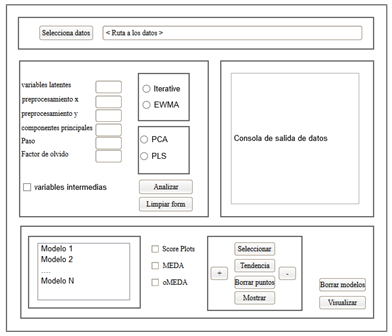
\includegraphics[width=0.7\textwidth]{imagenes/figuras/8_1.png}
\caption{Prototipo de la GUI.}
\end{figure}

\bigskip

En la etapa de análisis y especificación se pensó en una estructura con 3 paquetes o módulos diferentes que dependían unos de otros, pero para el desarrollo de la GUI se han aunado en una sola interfaz facilitando la comprensión por parte del usuario. Aun así siguen estando separadas las funciones de calibración del modelo, análisis y visualización mediante paneles separadores. El prototipo consta de diferentes subsecciones, que son la entrada de datos en la parte superior, la entrada de atributos para calibración del modelo a analizar en la parte intermedia izquierda, la consola de
salida en la parte intermedia derecha y las características de la visualización
en la parte inferior.
\bigskip

\section{Diseño de la arquitectura}

La integración de los 3 paquetes de la fase de análisis en uno sólo se ha hecho por simplicidad en el código ya que M no es el mejor lenguaje de programación para aplicar el paradigma de la orientación a objetos. La estructura de 3 paquetes se integró para separar las 3 partes conceptuales de la aplicación ya que los procesos que implican cada una de ellas son diferentes aunque dependan unos de otros. Como la estructura de datos que utilizan los 3 módulos es la misma, un Lmodel, no tendría tampoco mucho sentido crear 3 clases diferentes ya que lo único que las diferenciaría sería la función principal de cada una. Por lo tanto cada uno de los paquetes de la etapa de análisis se va a transformar en un módulo funcional y no en una clase propia, y todos ellos estarían integrados en un mismo fichero, compartiendo todos los datos del entorno de trabajo sin la necesidad de establecer mecanismos de transmisión de datos entre ellos más allá de la generación de variables globales.
\bigskip

\section{Diseño de los ficheros de código}
Se crearán dos ficheros para el desarrollo del software: GuiV1.fig y GuiV1.m.

\begin{itemize}
\item \textbf{Guiv1.fig:} contendrá la estructura de la interfaz gráfica. Como se explicó en capítulos anteriores GUIDE genera este tipo de ficheros para almacenar toda la parte de la GUI relacionada con la estética.
\item \textbf{Guiv1.m:} Este fichero tendrá almacenado todo el código propiamente dicho de la aplicación, tanto la integración con la interfaz gráfica como los métodos que le dan funcionalidad al programa.
\end{itemize}
\bigskip

\section{Diseño de los ficheros de datos para las pruebas}

Como lo que se desea analizar es BIG DATA la extensión de los ficheros de datos puede llegar a alcanzar un tamaño demasiado grande para los tamaños de ficheros de los sistemas (sobre todo en sistemas operativos de 32 bits), además la función load de Matlab saturaría la RAM con ficheros muy grandes, por lo que los ficheros de datos propiamente dichos se van a dividir en varios de tamaño más pequeño y se van a indexar con otro tipo de fichero. Por lo tanto se tendrán dos tipos de ficheros:

\bigskip

\begin{itemize}
\item \textbf{Ficheros de datos:} Almacenarán dos matrices, una bidimensional con los valores de X y otra unidimensional con los valores de las clases de cada una de las observaciones. Si es un modelo PLS también contendrá la matriz Y. Opcionalmente se pueden tener matrices con las observaciones y nombre de las variables.
\item \textbf{Ficheros índice:} Deberán tener al menos una matriz unidimensional con las rutas a cada uno de los ficheros de datos, y como parte opcional se puede añadir otra con los nombres de las variables a analizar.

\end{itemize}